\documentclass{jreport}
\usepackage{xcolor}
\usepackage{amsmath}
\usepackage{amsfonts}
\usepackage{amssymb}
\usepackage{amsthm}
\usepackage{bm}
\usepackage{romannum}
\usepackage[dvipdfmx,hidelinks]{hyperref}
\usepackage{pxjahyper}
\usepackage{framed}
\usepackage{pifont}
\usepackage[dvipdfmx]{graphicx}
\usepackage{float}
\newenvironment{claim}[1]{\par\noindent\underline{Claim:}\space#1}{}
\newenvironment{claimproof}[1]{\par\noindent\underline{Proof:}\space#1}{\hfill $\square$}
\DeclareMathOperator{\spn}{\mathbb{Q}-span}
\begin{document}
\pagenumbering{arabic}
\title{第11回演習課題解答}
\author{習近平}
\maketitle
\newpage
\tableofcontents
\newpage
\setcounter{chapter}{11}
\section{問題11.1}
\subsection{(1)$I$上一様収束する}
$$
f(x) =0
$$
\begin{figure}[H]
\centering
	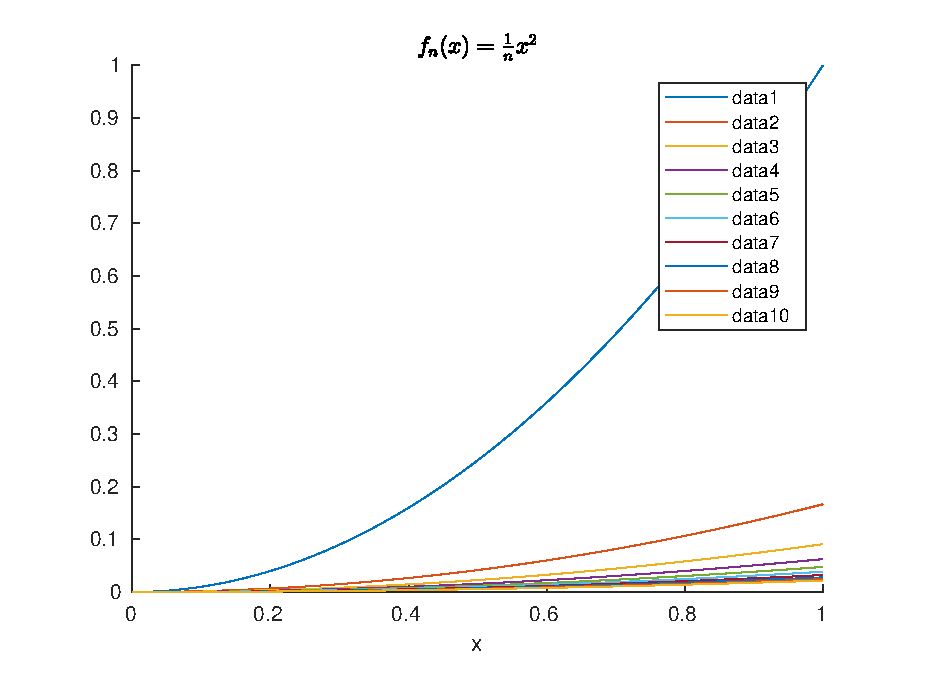
\includegraphics[scale=0.3]{1.eps}
\end{figure}
\subsection{(2)$I$上一様収束しない}
$$
f(x) = 0
$$
\begin{figure}[H]
	\centering
	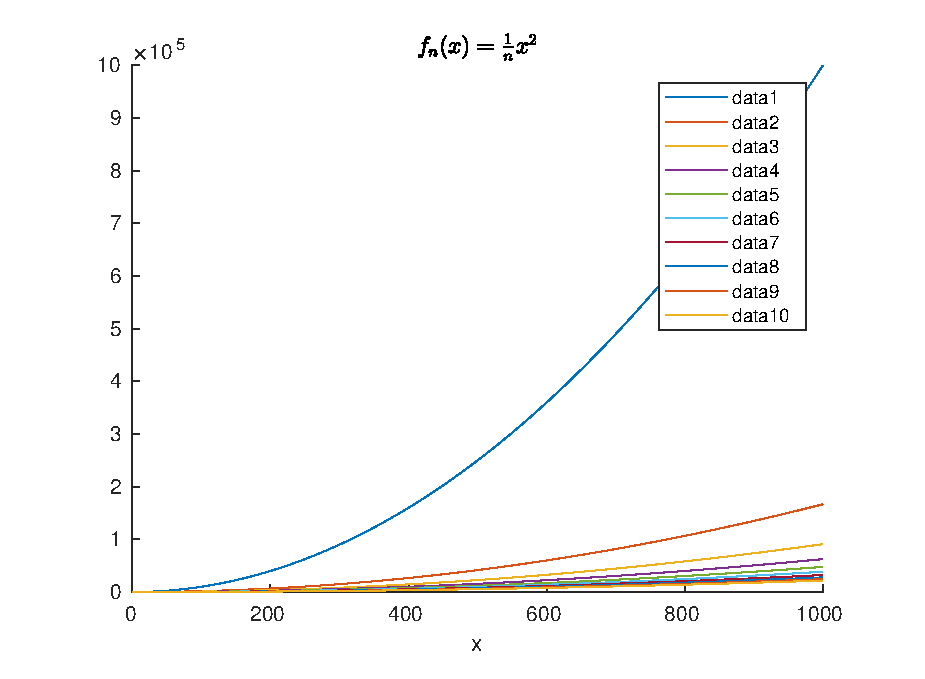
\includegraphics[scale=0.3]{2.eps}
\end{figure}
\subsection{(3)$I$上一様収束しない}
$$
f(x)=
\begin{cases}
	1,x=1\\
	0,x\neq 1
\end{cases}
$$
\begin{figure}[H]
	\centering
	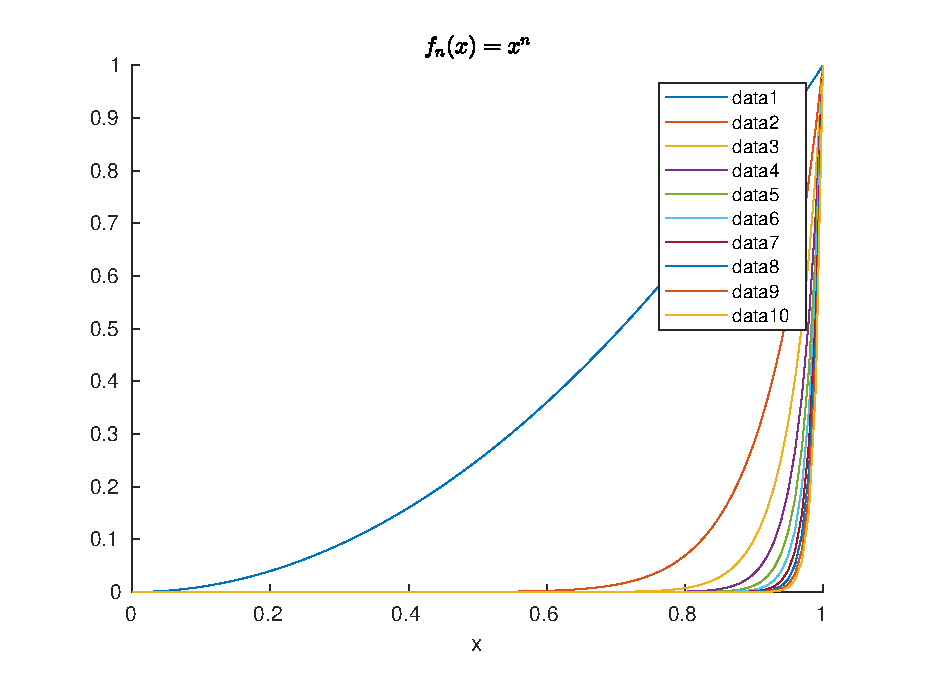
\includegraphics[scale=0.3]{3.eps}
\end{figure}
\subsection{(4)$I$上一様収束する}
$$
f(x) = 0
$$
\begin{figure}[H]
	\centering
	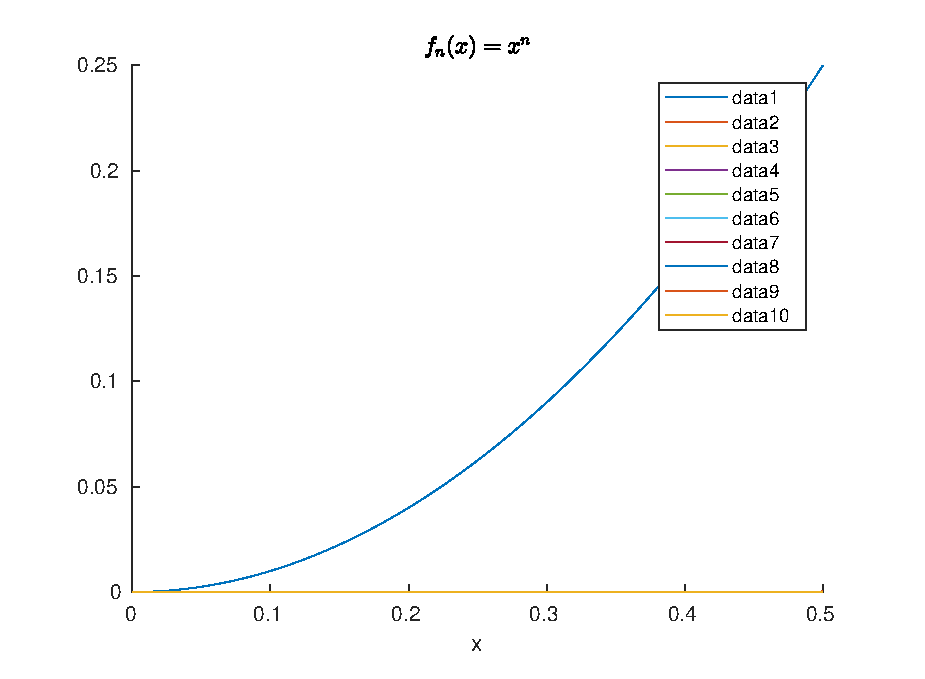
\includegraphics[scale=0.3]{4.eps}
\end{figure}
\subsection{(5)$I$上一様収束しない}
$$
f(x)=0
$$
\begin{figure}[H]
	\centering
	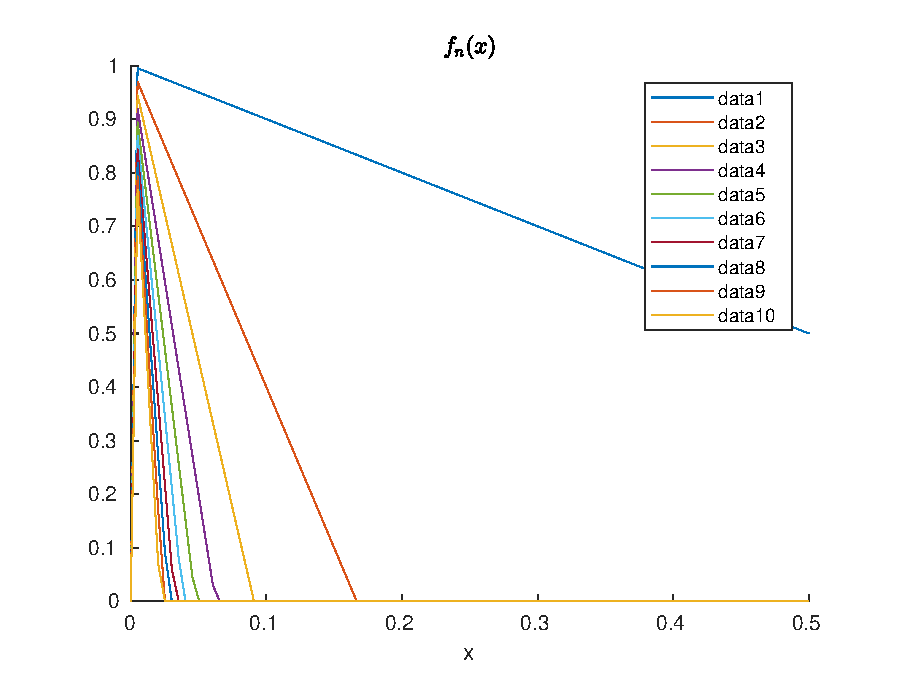
\includegraphics[scale=0.3]{5.eps}
\end{figure}
\subsection{(6)$I$上一様収束しない}
$$
f(x) =1
$$
\begin{figure}[H]
	\centering
	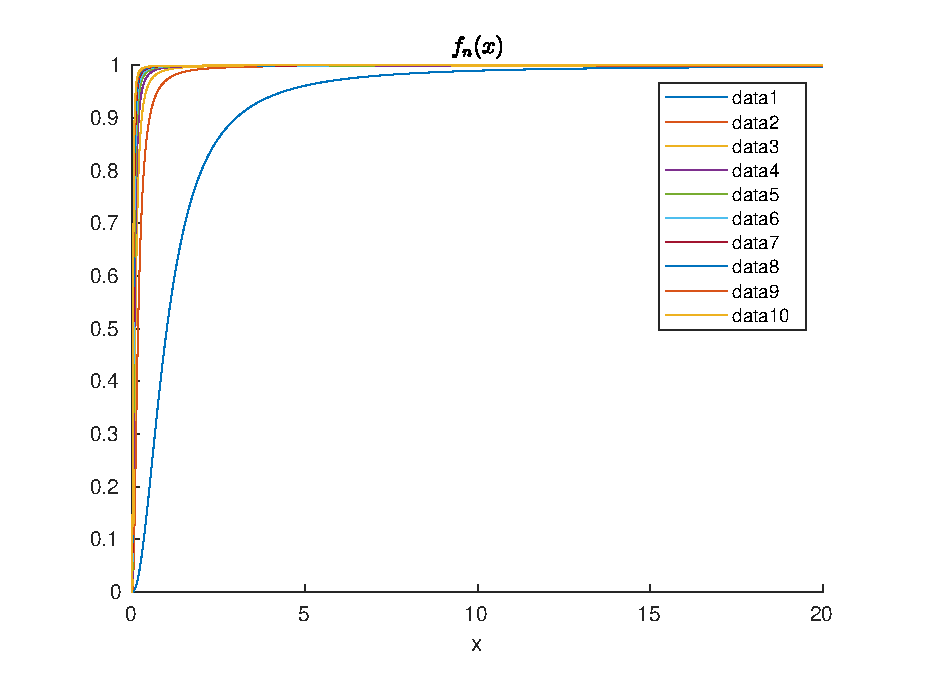
\includegraphics[scale=0.3]{6.eps}
\end{figure}
\newpage
\section{各$f_n$は区間$I$上連続であり,$(f_n)$が$I$上で$f$に一様収束とする.この時,$f$も$I$上連続である}
示すべきことは以下の論理式で表される命題である:
$$
 \forall a \in I; \forall \varepsilon \in \mathbb{R}_{>0}; \exists \delta \in \mathbb{R}_{>0}; \forall x  \in I;\left( |x-a|<\delta \implies |f(x) -f(a)| <\varepsilon \right)
$$
$a \in I , \varepsilon \in \mathbb{R}_{>0}$を任意に取る.この時,$\varepsilon_0 = \varepsilon /3$とする.\\
$(f_n)$が$I$上で$f$に一様収束することより,$\varepsilon_0 $に対し,ある自然数$N$が存在し,$n \ge N$を満たす任意の$n$に対し,任意の$x \in I$に関して,$| f_n(x) -f(x) |<\varepsilon_0$が成り立つ.\\
このような自然数$N,n$を一つずつ取る.\\
この自然数$n$に対し,$f_n$が$I$上で連続であることより,$a,\varepsilon_0$に対し,ある$\delta \in \mathbb{R}_{>0}$が存在し,$|x-a|<\delta$を満たす任意の$x \in I$に関して,$|f_n(x) - f_n(a)|<\varepsilon_0$が成立する.\\
このような$\delta \in \mathbb{R}_{>0}$を取る.\\
この時,$|x-a|<\delta$を満たす任意の$x \in I$に対し,先程の自然数$n$を用いて,以下の関係式が得られる:
\begin{equation}
	\begin{aligned}
		\left|f(x)-f(a)\right|&= \left|f(x)-f_n(x)+f_n(x)-f_n(a)+f_n(a)-f(a)\right| \\
				      &\le \left| f(x) - f_n(x) \right| + \left| f_n(x) - f_n(a) \right| +\left| f_n(a) -f(a) \right| \\
				      &<\varepsilon_0 +\varepsilon_0 +\varepsilon_0 =\varepsilon
	\end{aligned}
\end{equation}
以上より,命題が成り立つことを示せた.\\
\newpage
\section{\# 雑談}
最後の問題での$f_n$が一様連続ならば$f$も一様連続になるかな.とりあえずここまでしておいて,来週以降確認するとしよう.
\end{document}

